\secspace
\section{Introduction}
\label{sec:intro}

While many debate the ethical and legal issues around the training of
generative image models, all agree that their arrival has dramatically
disrupted a range of visual art industries, from fine art to illustrations,
concept art and graphics arts. Recent works has studied the harms experienced
by professional artists due to these large-scale image generators, including
reputational damage, economic loss, plagiarism and copyright
infringement~\cite{genaiimpact,genaiimpact2}.  One of the more harmful uses
of these image models is ``style mimicry,'' where someone ``finetunes'' a
model on small samples of a specific artist's art, then uses the result to
produce images in the artist's individual style without their
knowledge~\cite{hollie-steal,sarah-andersen,lensa-steal,sam-steal}. These
mimicry models (usually lightweight models known as LORAs) are hosted on
sites including Civitai, Tensor.art, PromptHero and HuggingFace.

Recently, the security and machine learning communities have developed a
number of tools to disrupt unauthorized style mimicry, including
Glaze~\cite{shan2023glaze}, Mist~\cite{mist}, and
Anti-Dreambooth~\cite{antidb}. These tools disrupt the mimicry process, by
modifying images so that they misrepresent themselves in a target model's
style feature space during finetuning, while constraining changes to
minimize visual impact to human eyes.  Since their introduction, they have
been adopted widely by artists across the globe, e.g. Glaze reports more
than 2.3 million downloads in a year~\cite{shan2023glazewebsite}. 

\begin{figure*}[t]
    \centering
    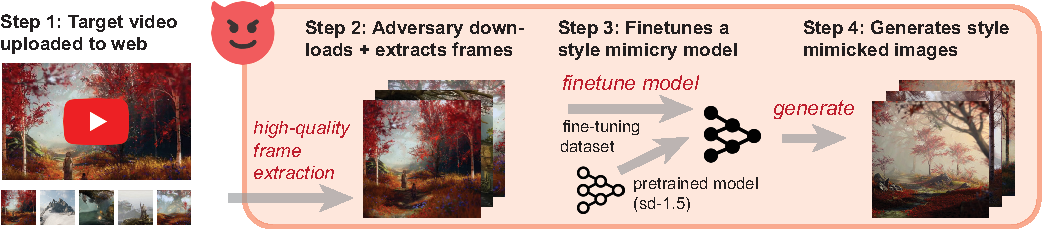
\includegraphics[width=0.75\textwidth]{plots/style-mimicry-scenario-eps-converted-to.pdf}
    \vspace{-0.1in}
    \caption{Style mimicry scenario demonstrating pipeline for adversaries to finetune a diffusion model on video frames}
    \label{fig:style-mimicry-scenario}
  \end{figure*}
  

There are signs, however, that mimicry attacks are shifting away from 2D art
images and towards video content (see Figure~\ref{fig:style-mimicry-scenario}). Online videos such as animations, game
cut-scenes, music videos and TV shows provide attractive sources
for training mimicry models for several reasons. First, a single video can
provide thousands of frames, each convertible to a standalone image for
training. For example, YouTube videos range from 30 to 60 frames per second,
and even a short 5 minute video can yield 18,000 frames for potential
training. Second, extracting frames from videos provides far more flexibility
to choose a specific scene, character or perspective. This offers far richer
training content compared to static images like movie posters or promotional
art. In fact, many new LORAs already target video games (Riot's League of
Legends\footnote{\url{https://huggingface.co/Totsukawaii/RiotDiffusion}} and
Valorant\footnote{\url{https://huggingface.co/ItsJayQz/Valorant_Diffusion}},
LucasArts
Games\footnote{\url{https://civitai.com/models/270789/lucasarts-games-style}},
Dead Or
Alive\footnote{\url{https://civitai.com/models/382550/kasumi-dead-or-alive-sdxl-lora-pony-diffusion}}),
TV shows (The
Flash\footnote{\url{https://civitai.com/models/42622/danielle-panabaker-the-flash-tv-show}},
Rick \&
Morty\footnote{\url{https://huggingface.co/Madhul/Rick_and_Morty_Stable_Diffusion_LORAS}}),
and movies (Hunger
Games\footnote{\url{https://civitai.com/models/160262/katniss-everdeen-hunger-games}},
Jumanji\footnote{\url{https://civitai.com/models/105883/ruby-roundhouse-from-jumanji-movies-karen-gillan}},
Disney Pixar\footnote{\url{https://tensor.art/models/662818547598142799}}). 


The natural question arises: {\em what can we do to protect video creators
  from style mimicry attacks?} This paper presents results from our efforts 
 to answer this question, and to disrupt style mimicry attacks on
video imagery. We begin by first validating the threat. Through empirical
experiments on a variety of short videos, we confirm that it is possible to
produce consistent, high quality mimicry models by extracting and training on
frames from videos. Next, we consider the feasibility of applying existing
tools like Glaze/Mist/Anti-DB to videos on a frame by frame basis. This naive
approach, while computationally expensive, does indeed protect against
extracting and training on video frames.

The problem, however, is that in the video domain, a naive application of
anti-mimicry tools is vulnerable to an adaptive countermeasure. Because
anti-mimicry tools are designed to operate on single images, they compute
protection filters on each single image independently. Randomized components
of these algorithms produce different optimization results on multiple runs
of the same image. For medium to high frame rate videos, this means a clever
attacker can take a protected video, extract consecutive frames whose originals are nearly identical, use the protected frames to identify alterations made by protection tools at the pixel level, and remove them to extract the original frames.  We explore multiple versions of this adaptive attack, and show that they can effectively bypass all 3 anti-mimicry tools and produce mimicry models similar in quality to those trained from
unprotected videos.

Next, we develop \system{}, an anti-mimicry framework for videos to resist this
countermeasure and restore robustness of anti-mimicry tools. At a high level,
we recognize commonalities across all 3 anti-mimicry tools, and extend these
tools to include the notion of sequential similar video frames. Instead of
computing a costly independent protection per frame, we first analyze video
frames to identify scenes or frame sequences with low pixel differential
across frames. The protection tool computes a single baseline perturbation
for all frames in the same scene, and then performs additional local
optimization on a per frame basis. The result is each new frame's protection
pixels is an extension from the prior frame, removing unnecessary
randomization used by the countermeasure. This new approach has the added
benefit of greatly reducing time required to generate protection, often by an
order of magnitude.

We evaluate the efficacy and robustness of \system{} on a variety of
videos. We validate that it integrates naturally with all 3 anti-mimicry
tools. We adapt \system{} to each tool and evaluate the robustness against
video mimicry attacks using multiple image-level metrics, including latent
$L_2$ norm between frames, intra-frame mean 
pixel difference, and CLIP-based genre shift.
Most importantly, we perform a
user study and ask participants to evaluate if the prototype is able to
provide sufficient protection against video mimicry attacks (including the
anti-mimicry countermeasure).  Responses from over 500 participants confirm that
not only does our robust anti-mimicry system works as intended against
mimicry models, but its protection is actually more visually appealing than
naive Glaze (less flickering due to randomization across frames).

Finally, we identify an advanced countermeasure against our frame-aggregation
framework, where an attacker can force us to break a sequence of similar
frames into multiple scenes. We show that even in these scenarios, frame
aggregation prevents an attacker from extracting unprotected frames. 

In summary, our paper makes the following contributions:
\begin{packed_itemize}
  \item We demonstrate that attackers can successfully mimic visual
    styles in videos by extracting and training on individual frames.
  \item We identify and validate the efficacy of an adaptive countermeasure
    that exploits randomization from per-image optimizations to remove image
    protection and enable successful mimicry.
  \item We propose a general anti-mimicry framework for videos that 
    aggregates scenes of similar frames into the protection process, removing
    unnecessary inter-frame randomization, reducing visual artifacts and
    greatly reducing computation costs.
  \item We validate the efficacy of our protection against mimicry attacks
    (including the adaptive countermeasure) using a variety of image metrics
    and two user studies of combined 525 participants.
  \item We propose another adaptive countermeasure on our framework,
    and show that it failures to extract unprotected frames for mimicry.
\end{packed_itemize}

Our work presents an important first step towards protecting video content
against visual style mimicry, by identifying and mitigating a video-specific
countermeasure to anti-mimicry tools. A number of challenges remain, and more
effort is needed to identify other adaptive mimicry algorithms, particularly
for longer videos. 